% This file was created with tikzplotlib v0.10.1.
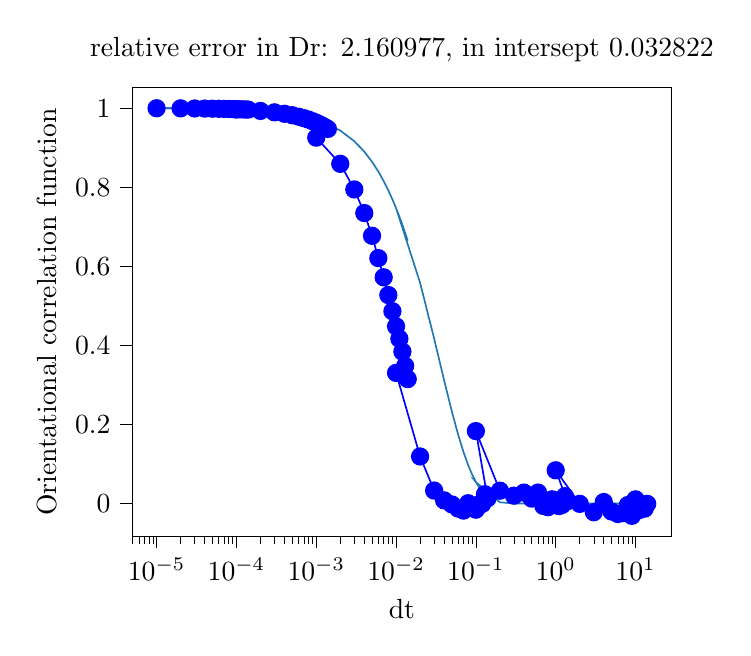
\begin{tikzpicture}

\definecolor{darkgray176}{RGB}{176,176,176}
\definecolor{steelblue31119180}{RGB}{31,119,180}

\begin{axis}[
log basis x={10},
tick align=outside,
tick pos=left,
title={relative error in Dr: 2.160977, in intersept 0.032822},
x grid style={darkgray176},
xlabel={dt},
xmin=4.92825984567174e-06, xmax=28.4075930214913,
xmode=log,
xtick style={color=black},
y grid style={darkgray176},
ylabel={Orientational correlation function},
ymin=-0.0827341354844826, ymax=1.051253408953,
ytick style={color=black}
]
\addplot [semithick, blue, mark=*, mark size=3, mark options={solid}]
table {%
1e-05 0.999703286561785
2e-05 0.999420072543146
3e-05 0.999139921983483
4e-05 0.998879711185157
5e-05 0.998630257132658
6e-05 0.998364306335462
7e-05 0.99810225582054
8e-05 0.997850197642064
9e-05 0.997593450627248
0.0001 0.997332289278215
0.00011 0.997078403808507
0.00012 0.996848883647003
0.00013 0.996603244362253
0.00014 0.996370457644791
0.0001 0.996533960860783
0.0002 0.992916226960677
0.0003 0.989359623261859
0.0004 0.985757577683576
0.0005 0.98209641298726
0.0006 0.978435415862982
0.0007 0.974696047298782
0.0008 0.970910708607475
0.0009 0.967018977992643
0.001 0.963077349107453
0.0011 0.959150439395097
0.0012 0.95521433521336
0.0013 0.951200206360856
0.0014 0.947422606035095
0.001 0.925362300924622
0.002 0.859172948676795
0.003 0.794309771377905
0.004 0.734601450280242
0.005 0.677145124052238
0.006 0.620630113934769
0.007 0.572098597073606
0.008 0.527281661347633
0.009 0.486330262075786
0.01 0.448021154518378
0.011 0.416600272680442
0.012 0.384090259818887
0.013 0.34795851442041
0.014 0.31463436588593
0.01 0.330265872588726
0.02 0.118922368677817
0.03 0.0327077330753731
0.04 0.00789084713699366
0.05 -0.00241667466297398
0.06 -0.0128527265841989
0.07 -0.0179911807450675
0.08 0.000661358824310369
0.09 -0.0065071078633806
0.1 -0.0156702533704326
0.11 -0.00219626621773343
0.12 -0.00112971475550121
0.13 0.0234160492980853
0.14 0.0132140747994203
0.1 0.183126829991302
0.2 0.032327861138557
0.3 0.0197233795581511
0.4 0.0274989731237936
0.5 0.0124421777023263
0.6 0.0276332762118389
0.7 -0.00624107160530615
0.8 -0.00937598023455149
0.9 0.0105412200778057
1 0.00694165523269228
1.1 -0.00653762798294646
1.2 -0.00373856703661117
1.3 0.0183606165284784
1.4 0.00559121479495769
1 0.0839823174475511
2 -0.00096701892012423
3 -0.0221033867227959
4 0.00366178244143635
5 -0.0202762319564379
6 -0.0265618234189682
7 -0.0243442279986381
8 -0.0040041292795212
9 -0.0311892471009605
10 0.0104807726639396
11 -0.0168781509725826
12 -0.0039944148273405
13 -0.0130285032267999
14 -0.000912785254375257
};
\addplot [semithick, steelblue31119180]
table {%
1e-05 0.99970852056948
2e-05 0.999417126099219
3e-05 0.999125816564453
4e-05 0.998834591940423
5e-05 0.998543452202381
6e-05 0.998252397325584
7e-05 0.997961427285297
8e-05 0.997670542056791
9e-05 0.997379741615347
0.0001 0.997089025936249
0.00011 0.996798394994792
0.00012 0.996507848766276
0.00013 0.996217387226009
0.00014 0.995927010349307
0.0001 0.997089025936249
0.0002 0.994186525642498
0.0003 0.991292474451822
0.0004 0.988406847769101
0.0005 0.985529621070811
0.0006 0.982660769904815
0.0007 0.979800269890157
0.0008 0.97694809671685
0.0009 0.974104226145677
0.001 0.971268634007976
0.0011 0.968441296205444
0.0012 0.965622188709925
0.0013 0.962811287563207
0.0014 0.960008568876824
0.001 0.971268634007976
0.002 0.94336275940772
0.003 0.916258658703931
0.004 0.889933295837348
0.005 0.864364296606157
0.006 0.839529929649928
0.007 0.815409087979898
0.008 0.791981271039925
0.009 0.769226567282849
0.01 0.747125637247457
0.011 0.725659697121676
0.012 0.704810502778012
0.013 0.684560334267675
0.014 0.664891980760208
0.01 0.747125637247457
0.02 0.558196717832419
0.03 0.417043078519985
0.04 0.311583575798885
0.05 0.232792077624583
0.06 0.173924929341426
0.07 0.129943773667432
0.08 0.0970843247076193
0.09 0.0725341879639191
0.1 0.0541921514047699
0.11 0.0404883456520994
0.12 0.0302498810464201
0.13 0.0226004616534663
0.14 0.0168853843149328
0.1 0.0541921514047699
0.2 0.0029367892738775
0.3 0.000159150928973874
0.4 8.62473123916195e-06
0.5 4.67392741138113e-07
0.6 2.5329018193247e-08
0.7 1.37263398886261e-09
0.8 7.4385988947776e-11
0.9 4.03113677545142e-12
1 2.18455974468599e-13
1.1 1.18385992436788e-14
1.2 6.41559162633836e-16
1.3 3.47674712765705e-17
1.4 1.88412406738089e-18
1 2.18455974468599e-13
2 4.77230127810253e-26
3 1.04253772616563e-38
4 2.2774859488979e-51
5 4.97530412305036e-64
6 1.08688491047859e-76
7 2.37436502253822e-89
8 5.18694224742739e-102
9 1.13311852317408e-114
10 2.47536511168419e-127
11 5.40758297638553e-140
12 1.18131880862606e-152
13 2.58066151496496e-165
14 5.63760926025292e-178
};
\end{axis}

\end{tikzpicture}
